\chapter{The Kakeya Problem in Finite Fields \label{chap:kakeya}}
Before we can discuss the Kakeya problem in finite fields, and its rather surprising resolution, we ought to first discuss the origin and history of the problem. 
Work on the Kakeya problem can be traced back to the Russian mathematician Abram Besicovitch in 1917. While working on a problem in Riemann integration, Besicovitch was led to consider the question of the existence of planar sets of measure zero which contain a line segment in every direction. In 1920, Besicovitch constructed such a set and published in a Russian Journal.

However, 1917 was a turbulent year as it marked the end of
the Russian Empire and the start of the Russian civil war. Due to this and the ensuing blockade of Russian ports there was scarce communication with the outside world.
Thus Besicovitch could not have known of a Japanese mathematician Kakeya who asked also in 1917 a related question: What is the smallest area of a convex set within which
one can rotate a needle by 180 degrees in the plane? Julius Pal answered this question in 1921 with the equilateral triangle in \cite{pal1920elementares}. The 
more interesting problem obtained by dropping the convexity condition remained open. In 1924, after leaving the newly formed Soviet Union for Copenhagen, Besicovitch discovered this
problem and by modifying his previous construction produced a solution in 1925. This lead to the more general questions being asked about Kakeya sets in higher dimensions.
\begin{definition}[Kakeya Set in $\RR^n$]
    A \textbf{Kakeya set} is a set $A \subset \RR^n$ that contains a unit segment in every direction.
\end{definition}
Besicovitch's construction showed that these sets can have arbitrarily small measures, even attaining zero, in $\RR^2$. Further, a straightforward process allows to extend the construction of these measure-zero sets to the case of arbitrary dimension.

Given that Kakeya sets can have measure zero, the natural question then arises, are Kakeya sets fractal in nature? This leads one to consider the dimension of Kakeya sets as a quantification of their fractal nature. There are many notions of dimensions that can be investigated, but we restrict ourselves to the Minkowski and Hausdorff dimensions.

\begin{definition}[Minkowski Dimension]
Given a set $S \subset \RR^n$, define $N(\varepsilon)$ to be the number of cubes of side length $\varepsilon$ required to cover the set.
The \textbf{Minkowski Dimension} of the set $S$ is then defined as
$$\dim_M (S) = \lim_{\varepsilon \to 0} \frac{\log( N(\varepsilon))}{\log (1/\varepsilon)}.$$
If this limit does not exist, one can still define the upper and lower Minkowski dimensions, 
$\dim_{M_{\text{upper}}}$ and $\dim_{M_{\text{lower}}}$, by taking the limit superior and limit inferior respectively.
\end{definition}
\begin{definition}[Hausdorff Dimension]
    We define the $d$-dimensional Hausdorff measure of a set $S \subset \RR^n$ as
    $$\mathcal{H}^d(S)=\lim_{r \to 0} \inf \left\{\sum_i r_i^d:\text{ there is a countable cover of } S\text{ by balls with radii } 0 < r_i < r\right\}.$$
    Then we can define the \textbf{Hausdorff dimension} of the set $S$ to be
    $$\dim_H (S) = \inf \{ d \geq 0 : \mathcal{H}^d(S) = 0 \}.   $$
\end{definition}
These dimensions are related by the following inequality when they are all defined:
$$\dim_H \leq \dim_{M_{\text{lower}}} \leq \dim_{M_{\text{upper}}}.$$
In 1971, Davies published \cite{davies1971some} showing that
although the measure of a Kakeya set in $\RR^2$ can be arbitrarily small, it must have Hausdorff and Minkowski dimension of 2.
This resulted in the following conjectures:
\begin{conjecture}[Kakeya Conjecture for the Minkowski Dimension]
    Let $A$ be a Kakeya set in $\RR^n$. Then $\dim_M (A) = n$. \label{conj:mink-kakeya}
\end{conjecture}
\begin{conjecture}[Kakeya Conjecture for the Hausdorff Dimension]
    Let $A$ be a Kakeya set in $\RR^n$. Then $\dim_H (A) = n$. \label{conj:haus-kakeya}
\end{conjecture}
In a survey on the problem, (see \cite{wolff1999recent}) Wolff proposed a finite analogue to the Kakeya Conjecture. We begin with some preliminaries so we can formally state this analogue.

\begin{definition}[Finite Field]
    A \textbf{finite field} $\FP$ is a field of finite cardinality. 
    The cardinality $|\FP| = q$ of a finite field is called the \textbf{order} of the finite field.
\end{definition}
It is known that finite field of order $q$ exists if and only if $q = p^k$ for some prime $p$ and integer $k$. For the rest of this chapter we let $q$ be of this form.

\begin{lemma}
    Each element $X$ in a finite field $\FF$ satisfies the identity:
    $$X^{|\FF|} - X =0$$
    identically in $\FF$. \label{lem:finite-fields-poly-identity}
\end{lemma}
\begin{proof}
    This lemma follows immediately from Fermat's Little Theorem.
\end{proof}


A Kakeya set in $\FP^n$ is a set that contains a line in every direction. In analogy to the Euclidean case, we formally define lines in $\FP^n$ as the sets of the form
$$\ell_{x,y} = \{x+ty :  t \in \FP \}$$
for some fixed $x,y \in \FP^n$ with $y\neq 0$.
It should be noted that a line in a finite field $\FP^n$ contains exactly $|\FP|$ points.
Formally, directions in $\FP^n$ can be identified using the projective space $\mathbb{P}\FP^n  = \FP^n/\FP^\times$. In this projective space, two lines $y$ and $y'$ are equivalent if $y'$ is a translation of $y$.
The finite analogue to Conjectures \ref{conj:mink-kakeya} and \ref{conj:haus-kakeya} is:
\begin{conjecture}[Kakeya Conjecture in Finite Fields]
    If $A\subset \FP^n$ contains a line in every direction, then $|A| \gtrsim_n |\FP|^n $. \label{KakeyaConjecture}
\end{conjecture}
This conjecture had a significant influence on the subject, inspiring work on the sum-product phenomenon in finite fields. From its postulation in 1999,
little progress was made in the following years and it was assumed that the problem was roughly as difficult as the Euclidean case. 

In 2008, Dvir published a remarkably simple proof of Conjecture \ref{KakeyaConjecture} using elementary facts about polynomials (See \cite{2008DVIR}). 
This proof revitalised interest in the polynomial method, and we shall explore its details later in this chapter. 

\begin{figure}[h]
\centering 
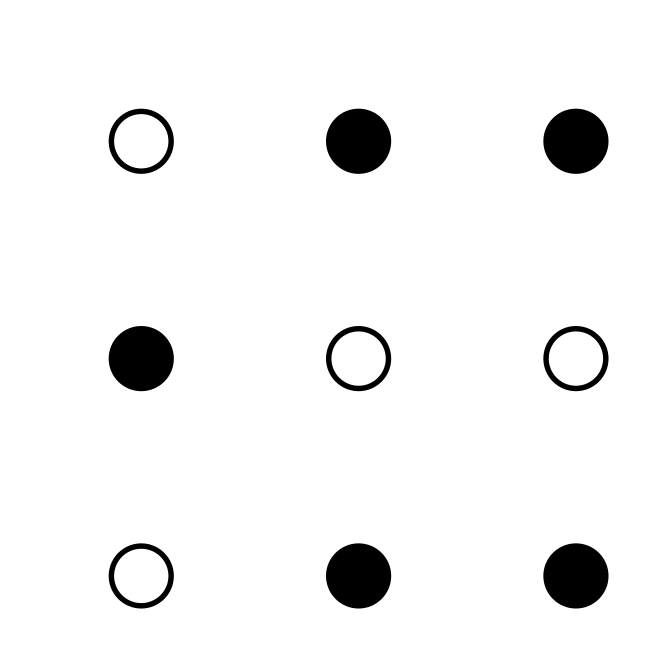
\includegraphics[width=0.3\textwidth]{images/kakeya_ex_f32.png}}
\caption{An example of a Kakeya set (shaded) in $\FF_3^2$.}
{\label{kak_ex_f32}
\end{figure}






\section{Combinatorial Attempts}
To truly show the power of the polynomial method, we shall first explore purely combinatorial attempts 
at estimating the sizes of Kakeya sets. All the following estimates are much weaker than the bound in Theorem \ref{KakeyaConjecture}.
We fix a finite field $\FF = \FF_{p^k}$ where $p$ is a prime. 

Our first estimate shows that Conjecture \ref{KakeyaConjecture} is true for the $n$ = 2 case.

\begin{lemma}
    Suppose $s \leq |\FF|$. If $l_1, \dots, l_s$ are distinct lines in $\FF^n$, then their union has cardinality at least $(1/2)|\FF|s$. \label{lem:kak-first-estimate}

    In particular, if $A \subset \FF^n$ is a Kakeya set, then we have
    \[
      |A| \gtrsim |\FF|^2.
    \] 
\end{lemma} 
\begin{proof}
    We add the lines together one at a time and track the cardinality of their union. The first line contains $|\FF|$ points. The second line must contain at least $|\FF| -1$ points not in the first line. Similarly the third line must contain at least $|\FF| -2$ points not in the first two lines, and so on. Thus the number of distinct points in the union of all $s$ lines is given by
    \[
      \sum_{i=1}^{s} |\FF| - i + 1  > (1/2) |\FF| s.
    \]

    A Kakeya set always contains at least $|\FF|$ lines, so setting $s=|\FF|$ above yields
    \[
        |A| > (1/2) |\FF|^2 .
    \]

\end{proof}

\subsection{Bush Argument} 
Bourgain produced one of the first non-trivial estimates of the dimension in his work \cite{BUSH1991}. We present the finite field analogue of his argument here (See \cite{GUTH2016}). This argument is known as the ``bush'' argument as we consider a high-multiplicity point through which pass many lines, forming a ``bush'' around that point. 


\begin{theorem}[Bush Argument]
If $A \subset \FF^n$ is a Kakeya set, then we have
$$|A| \gtrsim |\FF|^{\frac{n+1}{2}}.$$
\end{theorem}

\begin{proof}
    Let $\mu$ be a fixed multiplicity parameter to be chosen later. Either there exists a point $p\in A$ such that there are $\mu$ lines passing through $p$,
    or else every point in $A$ has less than $\mu$ lines passing through it.

    In the first case, since the lines have distinct directions they must become disjoint when $p$ is removed. Hence
    \[
      |A| \gtrsim \mu |\FF| .
    \]

    In the latter case, by double counting we have
    \begin{align*}
         \sum_{\ell \subset A} \sum_{p \in A} \OO[p \in \ell] &= \sum_{\ell \subset A} |\FF| = |\FF|^{n-1} |\FF| \\
        \sum_{p \in A} \sum_{\ell \subset A} \OO[p \in \ell] &\leq \sum_{p \in A} \mu = |A|\mu \\
        \implies \frac{|\FF|^{n}}{\mu} \leq |A|.
    \end{align*}
    Now we optimise the two lower bounds by choosing $\mu \sim |\FF|^{\frac{n-1}{2}}$, so that in either of the above cases we obtain
    \[
        |A| \gtrsim |\FF||\FF|^{\frac{n-1}{2}} \sim |\FF|^{\frac{n+1}{2}}.
    \]

\end{proof}

\subsection{Hairbrush Argument}
In \cite{WOLFF1995}, Wolff presented the ``hairbrush'' argument where he made an incremental improvement over the argument of Bourgain. It is similar in spirit to the ``bush'' argument above, 
however instead of using just one point of high-multiplicity we instead consider a line (or ``stem'') containing many points of high-multiplicity.

\begin{theorem}[Hair Brush Argument]
    If $A \subset \FF^n$ is a Kakeya set, then we have
    \[
        |A| \gtrsim |\FF|^{\frac{n+2}{2}}.
    \]
\end{theorem}
\begin{proof}
Let $\mu$ be a fixed multiplicity parameter to be chosen later. We say a line $\ell$ is $\mu$-rich if for at least $|\FF|/2$ points $p\in \ell$ there are $\mu$ lines distinct from $\ell$
in $A$ passing through $p$. Either there exists a $\mu$-rich line or there does not. 

Suppose a $\mu$-rich line exists, and denote this line by $\ell_\mu$. Consider the family $\Pi$ of 2-dimensional planes passing through $\ell_\mu$. 
If a line $\ell$ intersects $\ell_\mu$ then there exists a unique plane $\pi \in \Pi$ such that $\ell, \ell_\mu \in \pi$. 
Let $\LL_\pi := \{\ell \subset \pi \ | \ \ell \cap \ell_\mu \neq \emptyset \}$. The set $A \cap \pi$ is a set in (an isomorphic copy of) $\FF^2$ that contains at least $|\LL_\pi|$
lines, and hence by Lemma \ref{lem:kak-first-estimate} we have
\[
|A \cap \pi| \gtrsim |\LL_\pi| |\FF|.
\]
Thus,
\[
    |A| \geq \sum_{\pi \in \Pi} |(A \cap \pi) \backslash \ell_\mu| \gtrsim |\FF| \sum_{\pi \in \Pi} |\LL_\pi| \gtrsim \mu |\FF|^2,
\]
where the last inequality comes from the fact $\ell_\mu$ intersects at least $\mu |\FF|/2$ lines, so since the planes $\Pi$ foliate $\FF^n$, the union $\cup_\Pi \LL_\pi$ contains at least all of these lines.

Suppose there does not exist a $\mu$-rich line. Let 
\[
    A' = \{p \in A \ | \ p \text{ belongs to strictly less than } \mu \text{ lines in }A \}.
\]
Since we assume there does not exist a $\mu$-rich line in $A$, for any line $\ell \subset A$ we have $|A' \cap \ell| > |F|/2$. 
Proceeding by double counting, 
\begin{align*}
    |A| &\geq |A'|\geq \frac{1}{\mu} \sum_{p \in A'} \sum_{\ell \subset A} \OO[p \in \ell] \\
    &= \frac{1}{\mu} \sum_{\ell \subset A} |A' \cap \ell| \gtrsim \frac{1}{\mu} |\FF|^{n-1}|\FF|\\
    \implies |A| &\gtrsim \frac{|\FF|^n}{\mu}.
\end{align*}
Now optimising the two lower bounds by choosing $\mu \sim |\FF|^{\frac{n-2}{2}}$, so that in either of the above cases we obtain the bound
\[
    |A| \gtrsim |\FF|^2|\FF|^{\frac{n-2}{2}} \sim |\FF|^{\frac{n+2}{2}}.
\]
\end{proof}

\section{Dvir's Proof \label{sect:Dvirs-proof}}
Again we fix $\FF = \FF_{p^{q}}$ for some prime $p$.
\begin{theorem}[Kakeya Conjecture in Finite Fields]
    If $A\subset \FF^n$ contains a line in every direction, then $|A| \geq \frac{1}{n!} |\FF|^n $. \label{thm:Kakeya}
\end{theorem}
We shall prove this theorem via three surprisingly elementary lemmas. The general strategy of the proof is to assume the size of a Kakeya set $A$ is small and find a low-degree non-zero polynomial that interpolates (contains in its zero set) the points in $A$. We then show that due to the structure of the Kakeya set the polynomial's zero set must contain many more points. This contradicts the fact our polynomial is non-zero and of low-degree which  establishes the Kakeya Conjecture over finite fields.


The first lemma is a fundamental one to the polynomial method, exploiting the flexible interpolation properties of polynomials. 
Consider the problem of finding a non-zero polynomial in $\RR[X,Y,Z]$ of the minimal possible degree that vanishes at the points $(j,k, 2^{j^k})$ for $1\leq i \leq 10^{6}$. 
If we try to find an explicit polynomial we may produce
\begin{align*}
    P(X,Y,Z) &= \prod_{j,k=1}^{10^{6}} (X-j) (Y-k) 
    \intertext{or perhaps}
    Q(X,Y,Z) &= \prod_{j,k=1}^{10^{6}} (Z-2^{j^k}).
\end{align*}
Both $P$ and $Q$ vanish on our points and it is difficult to explicitly produce a polynomial of much lower degree that also satisfies this property.
One might consider taking the product of linear factors in $\RR[X,Y,Z]$, constructing the polynomial to vanish on sets of planes defined by three points in the collection.
Such a polynomial has a degree of $\lceil \frac{1}{3} 10^{12}\rceil $, which is slight improvement on 
$Q$ which has a degree of $10^{12}$. Naively one might conjecture that the degree of any polynomial with this property is of the order of $10^{12}$. 
Remarkably, the following lemma shows that we can find such a polynomial with a degree of about $\sim 18000$. This polynomial has roughly $\sim 18000^3$ coefficients and as such the polynomial is quite difficult to explicitly write, but we can establish the existence of such a polynomial non-constructively.
\begin{lemma}[Parameter Counting] 
Let $\KK$ be a (not necessarily finite) field. If $A \subset \KK^n$ and $|A| < {{n+D} \choose {n}}$, there exists a non-zero polynomial $P(X_1,\dots, X_n)$ of degree at most $D$ that vanishes on $A$. \label{lem:paramcounting}
\end{lemma}

\prf{ We first show the dimension of $\text{Poly}_D (\KK^n)$ is ${D+n} \choose{n}$. A basis for $\text{Poly}_D (\KK^n)$ is given by monomials of the form $X_1^{D_1}\dots X_n^{D_n}$, where $\sum_i D_i \leq D$, hence we just need to count the number of monomials.

We can map a monomial $X_1^{D_1}\dots X_n^{D_n}$ to a string of $D$ $\star$'s and $n$ $|$'s as follows. 
Begin with $D_1$ $\star$'s, then place one $|$. We put now $D_2$ $\star$'s, and place a second $|$. 
We continue until we have placed $D_n$ $\star$'s followed by an $n^{\text{th}}$ $|$. 
Finally we place $D - \sum_i D_i \star$'s.
 This is a bijective map between the monomials in $\text{Poly}_D (\KK^n)$ and all the strings of $D$ $\star$'s and $n$ $|$'s. 
 To assemble such a string we distribute the $n$ $|$'s over $n+D$ spaces, and then fill the remainder with $\star$'s. Hence we get the binomial coefficient
$$\text{Poly}_D (\KK^n) = {{n+D} \choose{n}}.$$

Now let $p_1, \dots, p_{|A|}$ be the points of $A$. We consider the evaluation map $E: \text{Poly}_D (\KK^n) \to \KK^{|A|}$ defined by
$$E(Q) = \left(Q(p_1), \dots, Q(p_{|A|})\right).$$

This map is clearly linear. 
Its kernel $\ker E$ is exactly the set of polynomials in $\text{Poly}_D (\KK^n)$ that vanish on $A$. 
By assumption, the dimension of $\text{Poly}_D (\KK^n)$ is greater than $A$, so the dimension of the domain of $E$ is greater than the codomain of $E$. By the rank-nullity theorem, we conclude $E$ must have a non-trivial kernel. 
Thus there exists a non-zero polynomial $P \in \text{Poly}_D (\KK^n)$ that vanishes on $A$.} 


Note that if $D=|\FF|-1$, and $|A| \leq {{|\FF|+n-1} \choose{|\FF|-1}} = { {|\FF|+n-1} \choose{n}}$ we have a polynomial of degree at most $|\FF|-1$ that vanishes on $A$. 
Since $\frac{|\FF|^n}{n!} < {{|\FF|+n-1} \choose{n}}$, we can certainly find such a polynomial when $|A| \leq \frac{|\FF|^n}{n!}$. The restriction of $D=|\FF|-1$ is somewhat necessary due to the fact that polynomials with a factor of $X^{|\FF|} - X$ vanish identically by Lemma \ref{lem:finite-fields-poly-identity}.



\begin{lemma}Suppose $A \subset \FF^n$ contains a line in every direction, and suppose that there exists a non-zero polynomial $P$ with degree $D<|\FF|$ that vanishes on $A$. Then there exists a non-zero degree $D$ polynomial $\bar{P}$ that vanishes everywhere on $\FF^n$. \label{lem:kaklem2} \end{lemma}

\prf{ Choose a line in $A$, say $\ell = \{x+ty : t\in \FF \}$ with $x,y\in \FF^n$ and $y \neq 0$. Now we consider the restriction of our polynomial $P$ to the line $\ell$, $P_{|\ell}$.
Recall $P$ is a sum of monomials, and we use multi-index notation here with $\alpha = (\alpha_1, \alpha_2, \dots, \alpha_n), \ \alpha_i \in \NN \cup \{0\}$ and $|\alpha| =  \sum \alpha_i$. $P$ can be written as
$$P(X_1,X_2, \dots, X_n) = \sum_{|\alpha| \leq D} c_{\alpha} X_1^{\alpha_1}X_2^{\alpha_2}\dots X_n^{\alpha_n}. $$
Now $P_{|\ell}$ can be written
$$P_{|\ell} = P(x+ty) = Q_{x,y}(t) = \sum_{|\alpha| \leq D} c_\alpha \prod_{i} (x_i + t y_i)^{\alpha_i}.$$
We now wish to examine the degree $D$ term of $Q$,
which consist in the terms of the expansion of the expression above obtained by the product of the $ty_i$ terms when $|\alpha| = D$. 
 
This is related to the degree $D$ component $Q_D$ of $Q$ by the identity
$$Q_{x,y,D} = t^D Q_D(y) = t^D \sum_{|\alpha| = D} c_\alpha \prod_i y_i^{\alpha_i}.$$

Now if $P_{|\ell}$ vanishes everywhere on $\ell$, since its dependence on $t$ is given by a polynomial of degree less than $|\FF|$, all its coefficients must be zero. In particular, we must have $Q_{x,y,D} = 0$.
This is clear from the factor theorem, as we could write the roots of $P_{|\ell}$ as $(t-k_1)(t-k_2)\dots(t-k_{|\FF|})$; but this contradicts the fact $P$ is of degree $D < |\FF|$.

Notice that $Q_{x,y,D}$ no longer depends on $x$, but on $y$ alone. In particular $Q_D(y) = 0$, but $y$ was an arbitrary non-zero element of $\FF^n$, and $Q_D(y)$ also vanishes at zero, so it vanishes everywhere. Thus we can pick $\bar{P}$ = $Q_D$, and we are done.
}

Finally, we show that any non-zero polynomial in $\FF[X_1, \dots, X_n]$ with degree less than $|\FF|$ cannot be zero everywhere in $\FF^n$.

\lem{Let $P$ be a non-zero polynomial on $\FF^n$ with degree less than $|\FF|$. Then $P$ does not vanish everywhere. \label{lem:kaklem3}}

\prf{ We proceed by induction on $n$. For $n=1$, a non-zero polynomial that vanishes everywhere has $|\FF|$ roots, so must be at least of degree $|\FF|$.
Let us assume that the statement holds in $\FF^{n-1}$, we now prove it must also hold for $\FF^n$.

We proceed by contradiction, assuming that $P$ vanishes everywhere. We let $X_1, \dots ,X_n$ be coordinates on $\FF^n$, and we write $P$ in the form

$$P(X_1, \dots ,X_n) = \sum_{j=n}^{|\FF|-1} P_j(X_1, \dots X_{n-1}) X_n^j.$$

Each $P_j$ are polynomials in $X_1, \dots X_{n-1}$ of degree less than $|\FF|$. Fix $X_1, \dots X_{n-1}$, and let $X_n$ vary. Now we have a polynomial in $X_n$ of degree less than $|\FF|$ that vanishes for all $X_n \in \FF$. By the base case this must be the zero polynomial. So each $P_j(x_1, \dots, x_{n-1}) = 0$ for all $j$ and for all $(x_1, \dots x_{n-1}) \in \FF^{n-1}$. Now by induction on $n$, each $P_j$ is the zero polynomial. Then $P$ is the zero polynomial as well. 
}
We now combine these lemmas to establish the Kakeya conjecture over finite fields.
\begin{proof} [Proof of Theorem \ref{thm:Kakeya}] 
Assume $A \subset \FF^n$ is a Kakeya set, and that $|A| \leq \frac{|\FF|^n}{n!}$. Then by Lemma \ref{lem:paramcounting} we can find a 
non-zero polynomial of degree at most $|\FF|-1$, say $P$, that vanishes on $A$. Now by Lemma \ref{lem:kaklem2} there exists a non-zero polynomial $\bar{P}$ that vanishes everywhere on $\FF^n$, and has degree less than $|\FF|$.
Finally, Lemma \ref{lem:kaklem3} says that such a $\bar{P}$ is necessarily the zero polynomial, a contradiction. We conclude that $|A| > \frac{|\FF|^n}{n!}$, or in other words
$$
|A| \gtrsim_n |\FF|^n.
$$
\end{proof}

\begin{remark}
    Theorem \ref{thm:Kakeya} lends a good degree of support for Conjectures \ref{conj:mink-kakeya} and \ref{conj:haus-kakeya} as it essentially rules out purely algebraic counter-examples.
\end{remark}